\documentclass{beamer}
\mode<presentation>
{
\usetheme{Madrid}
\usecolortheme{seagull}
}

\usepackage{graphicx}
\usepackage{amsmath}
\usepackage{amssymb}

\title[Inheritance]{Inheritance} 

\author{Jaime Canizales} 
\institute[Hunter College] 
{
City University of New York \\ 
\medskip
\textit{jaime.canizales@hunter.cuny.edu} 
}
\date{\today} 
\begin{document}


\begin{frame}
\titlepage 
\end{frame}


\begin{frame} \frametitle{Overview} 
\tableofcontents
\end{frame}


\section{Introduction}
\begin{frame}\frametitle{What is Inheritance?}
\begin{block}{Problem Statement}
    Inheritance is a mechanism in C++ which allows for you to pass 
    properties (attributes and methods), from one class to another. 
    The class whose properties and methods are inherited is known as the base class.
     And the class that inherits the properties from the parent class is the derived class.
\end{block}
\end{frame}


\begin{frame}\frametitle{Simple Example}
    \begin{figure}
        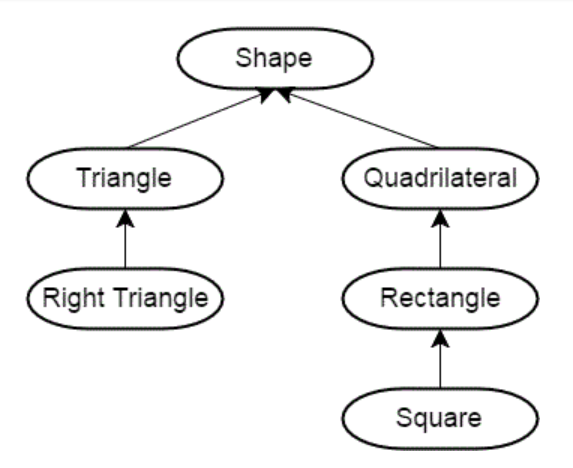
\includegraphics[width=10cm]{shapes.png}
    \end{figure}
    \end{frame}


\begin{frame}{Simple Example Cont.}
\begin{itemize}
\item Here we can see that both triangle and square are shapes. Therfore they can inherit properties
from the shape class. In this image we say that triangle and square are the derived classes and shape is the base class.
\item Right triangle is the derived class of triangle(base class), and triangle is the derived class
of shape(base class). This means the right triangle class inherits properties from both shape and triangle.
\end{itemize}
\end{frame}


\begin{frame}{Why use Inheritance?}
    \begin{itemize} 
    \item Allows us to write more concise code by reusing code from a pre-existing class.
    \item Can help in the understanding and implementation of polymorphism.
    \end{itemize}
    \end{frame}


\begin{frame}{What is Polymorphism?}
    \begin{itemize} 
    \item Polymorphism describes the concept that you can 
    access objects of different types through the same interface.
    \item This is computed at runtime in C++
    \end{itemize}
\end{frame}


\begin{frame}{Why use Polymorphism?}
    \begin{itemize} 
    \item For example, you have classes: BaseClass, DerivedClass1 and DerviedClass2, and they 
    all have a method doSomething(). The user presses a key "A", "S", or "D", and,
    depending on his input, an instance of the appropriate class is created, and
    its doSomething() method is called.
    \end{itemize}
\end{frame}


\section{Technical Information}
\begin{frame}{Constructors and Inheritance}
    \begin{itemize}
        \item When you create an instance of the derived class, the constructor for the base class
        must be called to initialize the data associated with the base class.
        \item You can set this up by adding the constructor you want to call for the base class in
        the member intialization list for the derived class.
        \item If you skip this step, the compiler will try to call the default constructor for the base class. 
        If there is no default constructor you will get a compiler error.  
    \end{itemize}
\end{frame}


\begin{frame}{Important Keywords}
    \begin{itemize}
    \item \textbf{virtual:} Allows for a function in the base class to be overwritten by
    functions of the same name in the derived class. 
    \item \textbf{override:} Ensure that a derived class overwrites a virtual function in the base class. 
    \end{itemize}  
    \end{frame}
    

\begin{frame}{Types of Inheritance}
    \begin{itemize}
        \item Public inheritance will inherit all the public properties of the base class 
        and make them public members of the derived class. Everyone has access to these members. 
        Syntax: \textbf{class derived: public base}
        \item Protected inheritance will inherit all the public properties of the base class 
        and make them protected members of the derived class. Protected means only the current class 
        and classes derived from the current class will have access to protected members.
        Syntax: \textbf{class derived: protected base}
        \item Private inheritance will inherit all the public properties of the base class 
        and make them private members of the derived class. Only the current class will
        have access to these members. Syntax: \textbf{class derived: private base}   
        \item If you do not choose an inheritance type, C++ defaults to private inheritance 
        (just like members default to private access if you do not specify otherwise). 
    \end{itemize}
\end{frame}


\begin{frame}{Technical things to keep in mind}
    \begin{itemize}
    \item If you implement a destructor, make sure base class is virtual.
    \item Virtual functions and polymorphism only works for pointers and references.
    \end{itemize}  
\end{frame}


\section{Conclusion}
\begin{frame}\frametitle{Software Architecture of Code Example}
\begin{figure}
    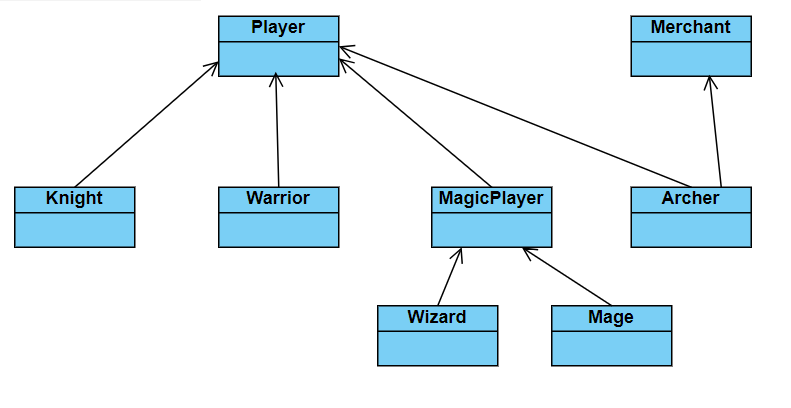
\includegraphics[width=12cm]{code.png}
\end{figure}
\end{frame}


% \begin{frame}
% \frametitle{References}
% \footnotesize{
% \begin{thebibliography}{99} 
% \bibitem[Urain, 2023]{p1} Julen Urain, Niklas Funk, Jan Peters, Georgia Chalvatzaki (2023)
% \newblock SE(3)-DiffusionFields: Learning smooth cost functions for joint grasp and motion optimization through diffusion
% %\newblock \emph{© Springer Science+Business Media, LLC, part of Springer Nature 2020}.
% \end{thebibliography}
% }
% \end{frame}



\end{document}
